~\\
\begin{center}
    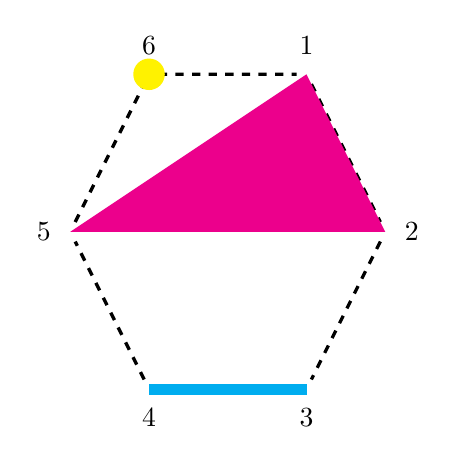
\begin{tikzpicture}[scale=1]
        \node [label = above : {$1$}] (1)
            at (4,5) {};
        \node [label = right : {$2$}] (2)
            at (5,3) {};
        \node [label = below : {$3$}] (3)
            at (4,1) {};
        \node [label = below : {$4$}] (4)
            at (2,1) {};
        \node [label = left : {$5$}]  (5)
            at (1,3) {};
        \node [label = above : {$6$}] (6)
            at (2,5) {};
        \draw [dashed][very thick]
        (1) -- (2) -- (3) -- (4)
            -- (5) -- (6) -- (1);
        \fill [color = magenta] (4,5) -- (5,3)
            -- (1,3) -- cycle;
        \draw [color = cyan][line width = 4pt] 
            (4,1) -- (2,1);
        \fill [color=yellow] (2,5) circle (0.2);
      \end{tikzpicture}
\end{center}